\section{Muh. Rifky Prananda (1174017)}
\subsection{Teori}
\subsubsection{Soal No. 1}
\hfill \break
Apa itu fungsi library matplotlib?

\hfill \break
Matplotlib adalah salah satu perpustakaan Python 2D yang dapat menghasilkan plot kualitas lebih tinggi dalam berbagai format dan dapat digunakan pada berbagai platform. Matplotlib berfungsi sebagai pembuat grafik di berbagai platform, seperti Jupyter dan Python.

\subsubsection{Soal No. 2}
\hfill \break
Jelaskan langkah-langkah membuat sumbu X dan Y di matplotlib!

\begin{enumerate}
	\item Pertama yaitu memasukkan atau mengimport library.	
	\lstinputlisting[firstline=2, lastline=2]{src/6/1174017/1174017.py}
	
	\item Selanjutnya menghasilkan nilai sumbu x dan sumbu y.	
	\lstinputlisting[firstline=4, lastline=5]{src/6/1174017/1174017.py}
	
	\item Kemudian membuat fungsi untuk mem-plot diagram batang.
	\lstinputlisting[firstline=7, lastline=7]{src/6/1174017/1174017.py}	

	\item Terakhir kita menampilkan plot nya.
	\lstinputlisting[firstline=9, lastline=9]{src/6/1174017/1174017.py}
	
\end{enumerate}
\hfill \break
\textbf{Kode Program}

\lstinputlisting[caption = Kode program membuat diagram menggunakan Matplotlib., firstline=2, lastline=9]{src/6/1174017/1174017.py}

\hfill \break
\textbf{Gambar yang dihasilkan}

\begin{figure}[H]
	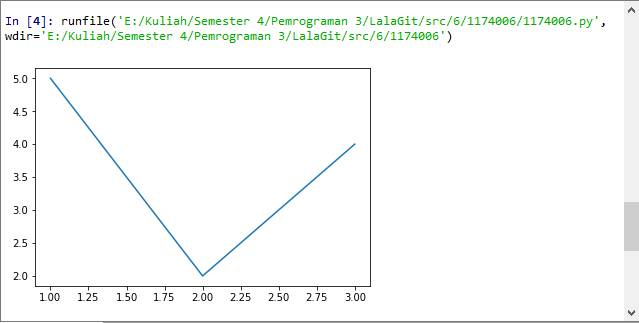
\includegraphics[width=12cm]{figures/6/1174017/2.png}
	\centering
	\caption{Diagram Batang}
\end{figure}
 
\subsubsection{Soal No. 3}
\hfill \break
Jelaskan bagaimana perbedaan fungsi dan cara pakai untuk berbagai jenis(bar, histogram ,scatter ,line, dll) jenis plot di matplotlib!

\begin{enumerate}
	\item \textbf{Bar Graph}
	
	Perbedaan antara grafik batang dan jenis plot lainnya adalah grafik batang menggunakan bar atau balok (batang) untuk membandingkan data antara berbagai kategori.
	
	\textbf{Kode Program}
	
	\lstinputlisting[caption = Kode program membuat bar graph menggunakan Matplotlib., firstline=2, lastline=9]{src/6/1174017/1174017.py}
	
	\textbf{Hasil Compile}
	
	\begin{figure}[H]
		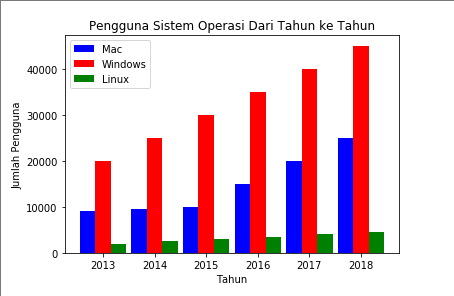
\includegraphics[width=12cm]{figures/6/1174017/bar.png}
		\centering
		\caption{Hasil compile membuat bar graph menggunakan Matplotlib.}
	\end{figure}
	
	\item \textbf{Histogram}
	
	Perbedaan antara histogram dan tipe plot lainnya adalah histogram akan membuat plot di mana plot yang diangkat adalah kombinasi dari beberapa data yang telah dikelompokkan.
	
	\textbf{Kode Program}
	
	\lstinputlisting[caption = Kode program membuat histogram menggunakan Matplotlib., firstline=29, lastline=36]{src/6/1174017/1174017.py}
	
	\textbf{Hasil Compile}
	
	\begin{figure}[H]
		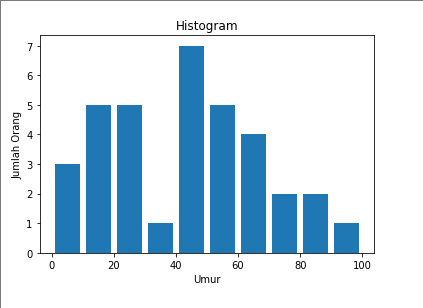
\includegraphics[width=12cm]{figures/6/1174017/histogram.png}
		\centering
		\caption{Hasil compile membuat histogram menggunakan Matplotlib.}
	\end{figure}
	
	\item \textbf{Scatter Plot}
	
	Perbedaan antara Scatter plot dan jenis plot lainnya adalah bahwa scatter plot menampilkan data sebagai kumpulan titik, yang masing-masing memiliki nilai satu variabel yang menentukan posisi pada sumbu horizontal dan nilai variabel lain menentukan posisi pada sumbu vertikal.
	
	\textbf{Kode Program}
	
	\lstinputlisting[caption = Kode program membuat scatter plot menggunakan Matplotlib., firstline=40, lastline=53]{src/6/1174017/1174017.py}
	
	\textbf{Hasil Compile}
	
	\begin{figure}[H]
		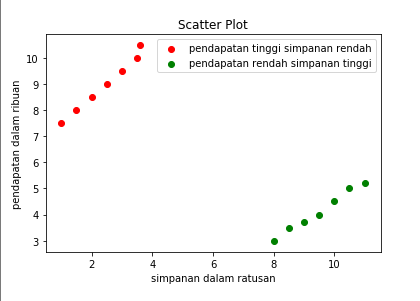
\includegraphics[width=12cm]{figures/6/1174017/scatter.png}
		\centering
		\caption{Hasil compile membuat scatter plot menggunakan Matplotlib.}
	\end{figure}
	
	\item \textbf{Area Plot}
	
	Perbedaan area plot dengan tipe plot lain adalah area plot dapat digunakan buat melacak perubahan dari waktu ke waktu untuk dua atau lebih kelompok terkait yang dapat membentuk satu kategori secara menyeluruh.
	
	\textbf{Kode Program}
	
	\lstinputlisting[caption = Kode program membuat diagram menggunakan Matplotlib., firstline=57, lastline=76]{src/6/1174017/1174017.py}
	
	\textbf{Hasil Compile}
	
	\begin{figure}[H]
		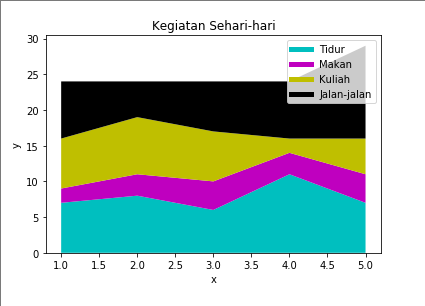
\includegraphics[width=12cm]{figures/6/1174017/area.png}
		\centering
		\caption{Hasil compile membuat diagram menggunakan Matplotlib.}
	\end{figure}
	
	\item \textbf{Pie Plot}
	
	Perbedaan pie plot dengan jenis plot yang lainnya yaitu pie plot digunakan untuk bisa menunjukkan presentase atau data proporsional di mana di setiap potongan pie dapat mewakili kategori.
	
	\textbf{Kode Program}
	
	\lstinputlisting[caption = Kode program membuat Pie Plot menggunakan Matplotlib., firstline=80, lastline=101]{src/6/1174017/1174017.py}
	
	\textbf{Hasil Compile}
	
	\begin{figure}[H]
		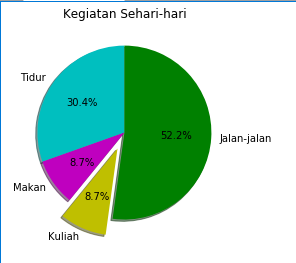
\includegraphics[width=9cm]{figures/6/1174017/pie.png}
		\centering
		\caption{Hasil compile membuat Pie Plot menggunakan Matplotlib.}
	\end{figure}
	
	\item \textbf{Line Graph}
	
	Perbedaan line graph dengan jenis plot lain adalah line graph menampilkan diagram dalam bentuk garis.
	
	\textbf{Kode Program}
	
	\lstinputlisting[caption = Kode program membuat diagram menggunakan Matplotlib., firstline=105, lastline=113]{src/6/1174017/1174017.py}
	
	\textbf{Hasil Compile}
	
	\begin{figure}[H]
		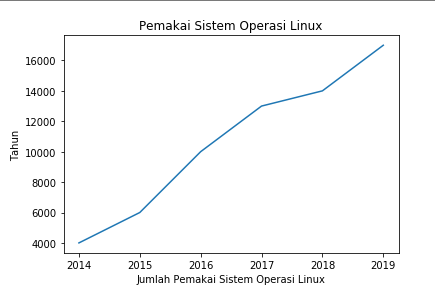
\includegraphics[width=12cm]{figures/6/1174017/line.png}
		\centering
		\caption{Hasil compile membuat diagram menggunakan Matplotlib.}
	\end{figure}
	
\end{enumerate}

\subsubsection{Soal No. 4}
\hfill \break
Jelaskan bagaimana cara menggunakan legend dan label serta kaitannya dengan fungsi tersebut!

\textbf{Legend}
Legend merupakan pendefinisian garis yang dilengkapi dengan sampel garis yang dijelaskan. Untuk bisa membuat legenda pada plot kita dapat menggunakan syntax fungsi legend pada MATLAB. 

\textbf{Label}
Untuk menambah label pada garis sumbu pada grafik dapat menggunakan syntax fungsi xlabel dan fungsi ylabel pada MATLAB. Kedua label ditulis setelah syntax deklarasi plot.

\subsubsection{Soal No. 5}
\hfill \break
Jelaskan apa fungsi dari subplot di matplotlib, dan bagaimana cara kerja dari fungsi subplot, sertakan ilustrasi dan gambar sendiri dan apa parameternya jika ingin menggambar plot dengan 9 subplot di dalamnya!

\hfill \break
Fungsi suatu subplot yaitu untuk membuat beberapa plot di dalam satu gambar.
\hfill \break
Cara kerja subplot, yaitu fungsi subplot memiliki parameter pertama adalah jumlah kolom, parameter kedua adalah jumlah baris, dan parameter ketiga adalah index plot keberapanya.

\hfill \break
\textbf{Kode Program}

\lstinputlisting[caption = Kode program membuat subplot menggunakan Matplotlib., firstline=134, lastline=146]{src/6/1174017/1174017.py}

\hfill \break
\textbf{Hasil Compile}

\begin{figure}[H]
	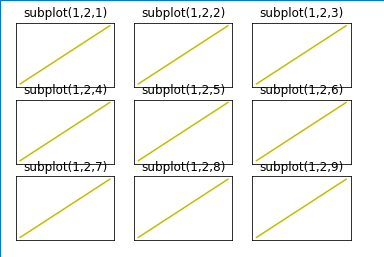
\includegraphics[width=12cm]{figures/6/1174017/subplot.png}
	\centering
	\caption{Hasil compile membuat subplot menggunakan Matplotlib.}
\end{figure}

\subsubsection{Soal No. 6}
\hfill \break
Sebutkan semua parameter color yang bisa digunakan (contoh:  m,c,r,k,...  dkk)!

\begin{itemize}
	\item 'b' (blue)
	\item 'g' (green)
	\item 'r' (red)
	\item 'c' (cyan)
	\item 'm' (magenta)
	\item 'y' (yellow)
	\item 'k' (black)
	\item 'w' (white)
\end{itemize}

\subsubsection{Soal No. 7}
\hfill \break
Jelaskan bagaimana cara kerja dari fungsi hist, sertakan ilustrasi dan gambar sendiri!

\hfill \break
Cara kerja dari sebuah fungsi hist adalah fungsi hist akan menerima parameter yang telah diberikan, selanjutnya fungsi hist akan bekerja sesuai dengan parameter yang diberikan.

\hfill \break
\textbf{Kode Program}

\lstinputlisting[caption = Kode program membuat diagram menggunakan Matplotlib., firstline=150, lastline=157]{src/6/1174017/1174017.py}

\hfill \break
\textbf{Hasil Compile}

\begin{figure}[H]
	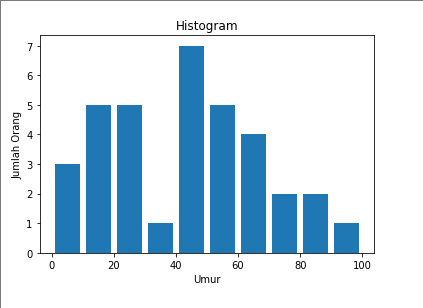
\includegraphics[width=12cm]{figures/6/1174017/histogram.png}
	\centering
	\caption{Hasil compile membuat diagram menggunakan Matplotlib.}
\end{figure}

\subsubsection{Soal No. 8}
\hfill \break
 Jelaskan lebih mendalam tentang parameter dari fungsi pie diantaranya labels, colors, startangle, shadow, explode, autopct!
 
 \begin{itemize}
 	\item labels : yaitu untuk memberi label di setiap persentase.
 	\item colors : yaitu untuk memberikan warna di tiap persentase.
 	\item startangle : yaitu untuk memutar plot sesuai dengan derajat yang ditentukan.
 	\item shadow : yaitu untuk memberikan bayangan pada plot.
 	\item explode : yaitu untuk memisahkan antar tiap potongan pie di plot.
 	\item autopct : yaitu untuk menentukan jumlah angka yang berada dibelakang koma.
 \end{itemize}

\subsection{Praktek}
\subsubsection{Soal No. 1}
\hfill \break
Buatlah librari fungsi (file terpisah/library dengan nama NPMbar.py) untuk plot dengan jumlah subplot adalah NPM mod 3 + 2!

\hfill \break
\textbf{Kode Program}

\lstinputlisting[caption = Kode program membuat fungsi Bar Plot menggunakan Matplotlib., firstline=1, lastline=21]{src/6/1174017/1174017_bar.py}

\hfill \break
\textbf{Hasil Compile}

\begin{figure}[H]
	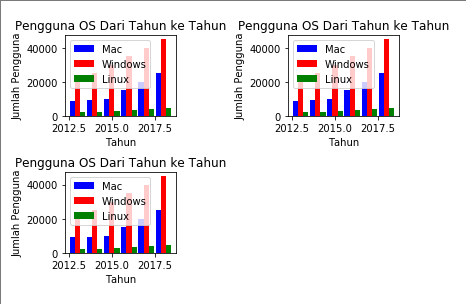
\includegraphics[width=12cm]{figures/6/1174017/p1.png}
	\centering
	\caption{Hasil compile membuat fungsi Bar Plot menggunakan Matplotlib.}
\end{figure}

\subsubsection{Soal No. 2}
\hfill \break
Buatlah librari fungsi (file terpisah/library dengan nama NPMscatter.py) untuk plot dengan jumlah subplot NPM mod 3 + 2!

\hfill \break
\textbf{Kode Program}

\lstinputlisting[caption = Kode program membuat fungsi Scatter Plot menggunakan Matplotlib., firstline=1, lastline=23]{src/6/1174017/1174017_scatter.py}

\hfill \break
\textbf{Hasil Compile}

\begin{figure}[H]
	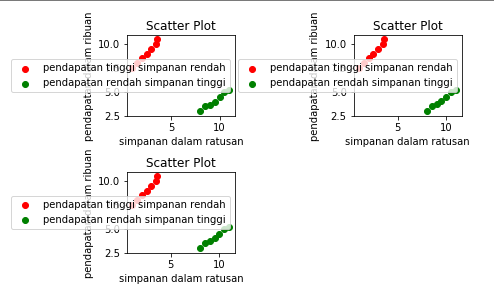
\includegraphics[width=12cm]{figures/6/1174017/p2.png}
	\centering
	\caption{Hasil compile membuat fungsi Scatter Plot menggunakan Matplotlib.}
\end{figure}

\subsubsection{Soal No. 3}
\hfill \break
Buatlah librari fungsi (file terpisah/library dengan nama NPMpie.py) untuk plot dengan jumlah subplot NPM mod 3 + 2!

\hfill \break
\textbf{Kode Program}

\lstinputlisting[caption = Kode program membuat fungsi Pie Plot menggunakan Matplotlib., firstline=1, lastline=23]{src/6/1174017/1174017_pie.py}

\hfill \break
\textbf{Hasil Compile}

\begin{figure}[H]
	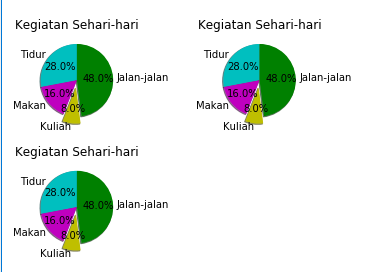
\includegraphics[width=12cm]{figures/6/1174017/p3.png}
	\centering
	\caption{Hasil compile membuat fungsi Pie Plot menggunakan Matplotlib.}
\end{figure}

\subsubsection{Soal No. 4}
\hfill \break
Buatlah librari fungsi (file terpisah/library dengan nama NPMplot.py) untuk plot dengan jumlah subplot NPM mod 3 + 2

\hfill \break
\textbf{Kode Program}

\lstinputlisting[caption = Kode program membuat fungsi Plot menggunakan Matplotlib., firstline=1, lastline=23]{src/6/1174017/1174017_plot.py}

\hfill \break
\textbf{Hasil Compile}

\begin{figure}[H]
	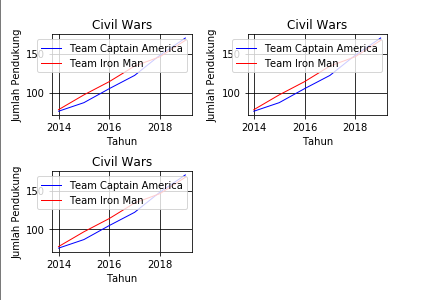
\includegraphics[width=12cm]{figures/6/1174017/p4.png}
	\centering
	\caption{Hasil compile membuat fungsi Plot menggunakan Matplotlib.}
\end{figure}


\subsection{Penanganan Error}
Tuliskan  peringatan  error  yang  didapat  dari  mengerjakan  praktek  keenam  ini, dan  jelaskan  cara  penanganan  error  tersebut. dan  Buatlah  satu  fungsi  yang menggunakan try except untuk menanggulangi error tersebut.

\hfill \break
Peringatan error di praktek kelima ini, yaitu:
\begin{itemize}
	\item Syntax Errors
	Syntax Errors adalah suatu keadaan saat kode python mengalami kesalahan penulisan. Solusinya adalah memperbaiki penulisan kode yang salah.
	
	\item Name Error
	NameError adalah exception yang terjadi saat kode melakukan eksekusi terhadap local name atau global name yang tidak terdefinisi. Solusinya adalah memastikan variabel atau function yang dipanggil ada atau tidak salah ketik.
	
	\item Type Error
	TypeError adalah exception yang akan terjadi apabila pada saat dilakukannya eksekusi terhadap suatu operasi atau fungsi dengan type object yang tidak sesuai. Solusi dari error ini adalah mengkoversi varibelnya sesuai dengan tipe data yang akan digunakan.
\end{itemize}
\hfill \break
Fungsi yang menggunakan try except untuk menanggulangi error.

\hfill \break
\textbf{Kode Program}

\lstinputlisting[caption = Kode program membuat fungsi penanganan error., firstline=161, lastline=178]{src/6/1174017/1174017.py}

\hfill \break
\textbf{Hasil Compile}

\begin{figure}[H]
	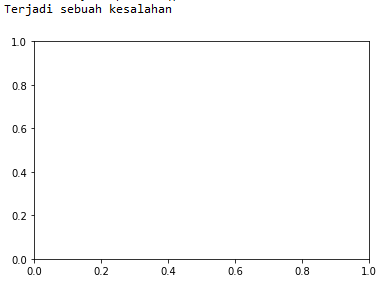
\includegraphics[width=12cm]{figures/6/1174017/error.png}
	\centering
	\caption{Hasil compile membuat fungsi penanganan error.}
\end{figure}